\documentclass[10pt,twocolumn,letterpaper]{article}

\usepackage[top=0.70in,bottom=0.78in,left=0.72in,right=0.72in,
            columnsep=0.28in]{geometry}
\usepackage{iftex}
\ifXeTeX
  \usepackage[UTF8,fontset=fandol]{ctex}
  \usepackage{fontspec}
  \setmainfont{Times New Roman}
  \CJKsetecglue{}
  \xeCJKsetup{CJKglue={\hskip 0pt}}
\else
  \usepackage[T1]{fontenc}
  \usepackage[utf8]{inputenc}
  \usepackage{times}
\fi
\usepackage{graphicx}
\usepackage{caption}
\usepackage{fvextra}
\usepackage{xurl}
\usepackage[hidelinks]{hyperref}
\usepackage{titling}
\usepackage{indentfirst}

\captionsetup{font=small,labelfont=bf}
\renewcommand{\figurename}{Figure}
\renewcommand{\tablename}{Table}
\setlength{\parindent}{1em}
\setlength{\parskip}{0.35em}
\setlength{\textfloatsep}{8pt plus 2pt minus 2pt}
\setlength{\floatsep}{7pt plus 2pt minus 2pt}
\setlength{\intextsep}{7pt plus 2pt minus 2pt}
\tolerance=1400
\emergencystretch=2em
\raggedbottom
\renewcommand{\thesection}{\arabic{section}.}
\renewcommand{\thesubsection}{\arabic{section}.\arabic{subsection}}
\makeatletter
\renewcommand\section{\@startsection{section}{1}{\z@}%
  {-2.0ex plus -0.5ex minus -0.2ex}%
  {0.7ex plus 0.2ex}%
  {\normalfont\large\bfseries\raggedright}}
\makeatother
\setlength{\droptitle}{-0.65in}
\pretitle{\begin{center}\fontsize{22}{24}\selectfont\bfseries}
\posttitle{\par\end{center}\vskip 0.45em}

\title{The Design of a\\
Practical System for\\
Fault-Tolerant Virtual Machines}
\author{Daniel J. Scales, Mike Nelson, and Ganesh Venkitachalam\\
VMware, Inc.\\
\texttt{\{scales,mnelson,ganesh\}@vmware.com}}
\date{}

\newcommand{\insertfigureone}{%
  \begin{figure}[t]
    \centering
    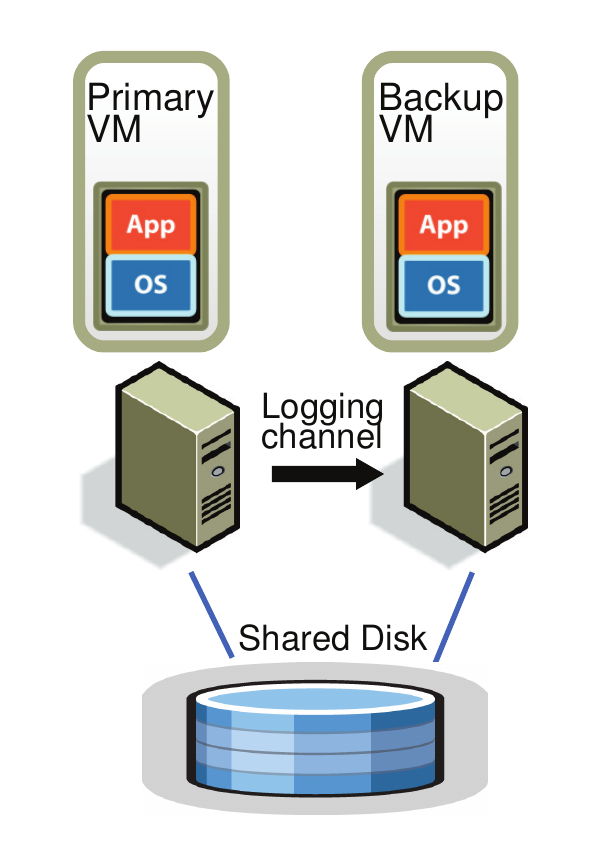
\includegraphics[width=0.56\columnwidth]{figures/original/figure-1-basic-ft.png}
    \caption{基本FT配置。}
  \end{figure}}
\newcommand{\insertfiguretwo}{%
  \begin{figure}[t]
    \centering
    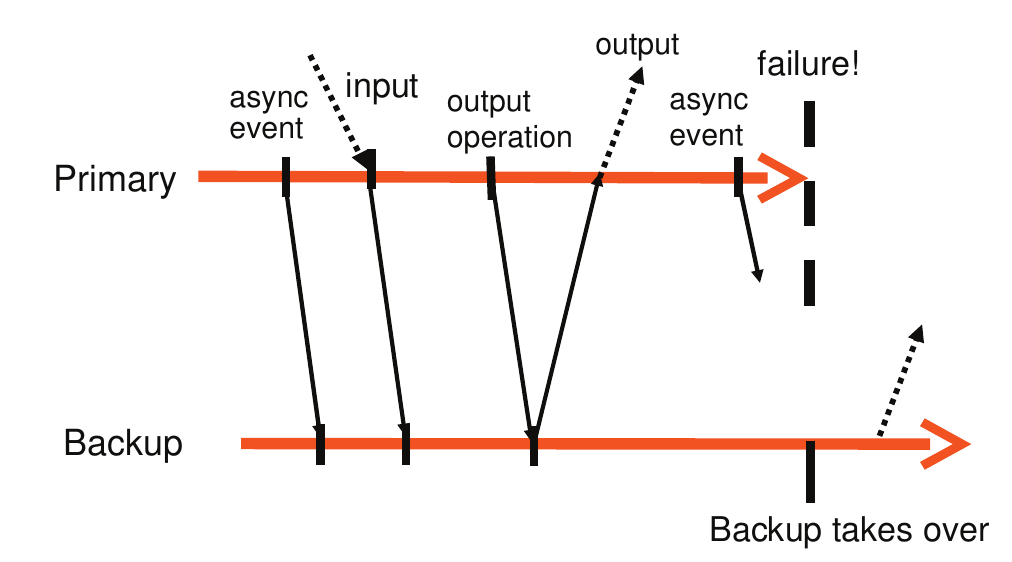
\includegraphics[width=0.95\columnwidth]{figures/original/figure-2-ft-protocol.png}
    \caption{FT协议。}
  \end{figure}}
\newcommand{\insertfigurethree}{%
  \begin{figure}[t]
    \centering
    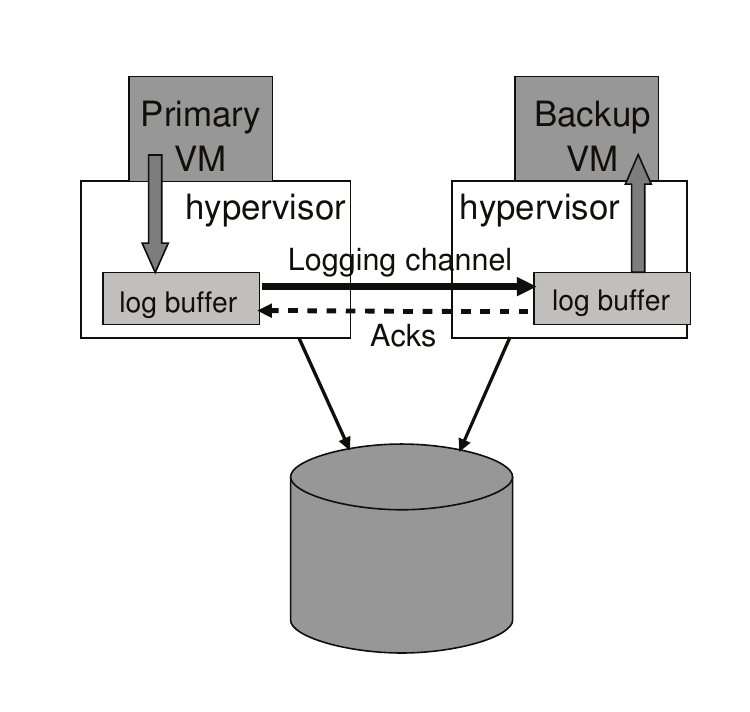
\includegraphics[width=0.95\columnwidth]{figures/original/figure-3-logging-buffers.png}
    \caption{FT日志缓冲区和通道。}
  \end{figure}}
\newcommand{\insertfigurefour}{%
  \begin{figure}[t]
    \centering
    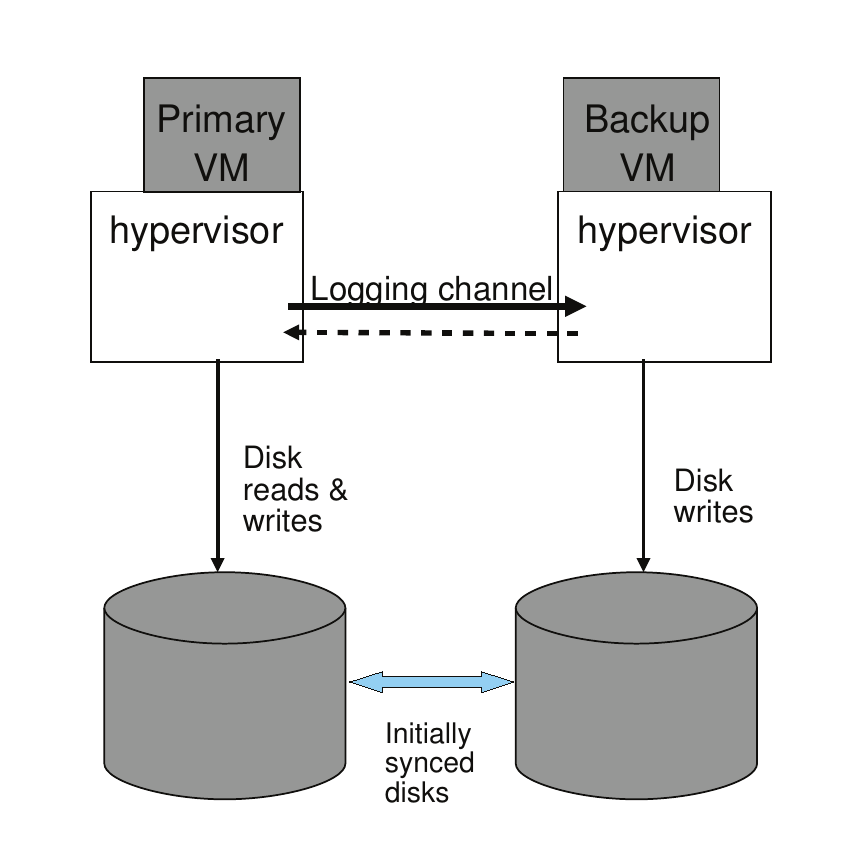
\includegraphics[width=0.95\columnwidth]{figures/original/figure-4-nonshared-disk.png}
    \caption{FT非共享磁盘配置。}
  \end{figure}}
\newcommand{\inserttableone}{%
  \begin{table}[t]
    \centering
    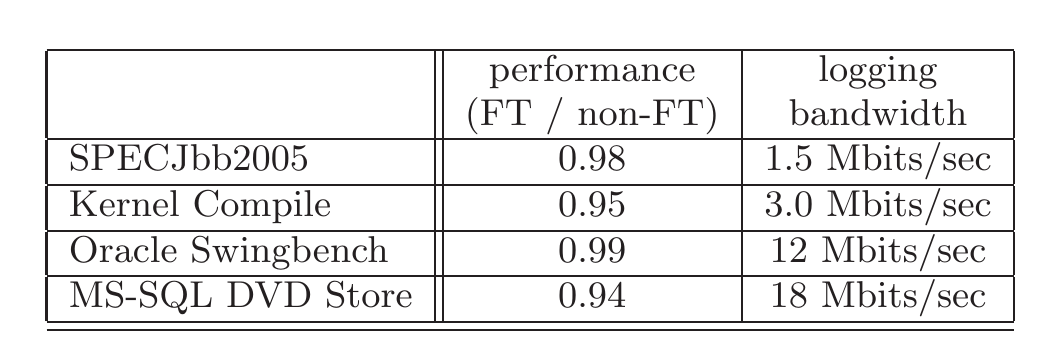
\includegraphics[width=\columnwidth]{figures/original/table-1-performance.png}
    \caption{基本性能结果。}
  \end{table}}
\newcommand{\inserttabletwo}{%
  \begin{table}[t]
    \centering
    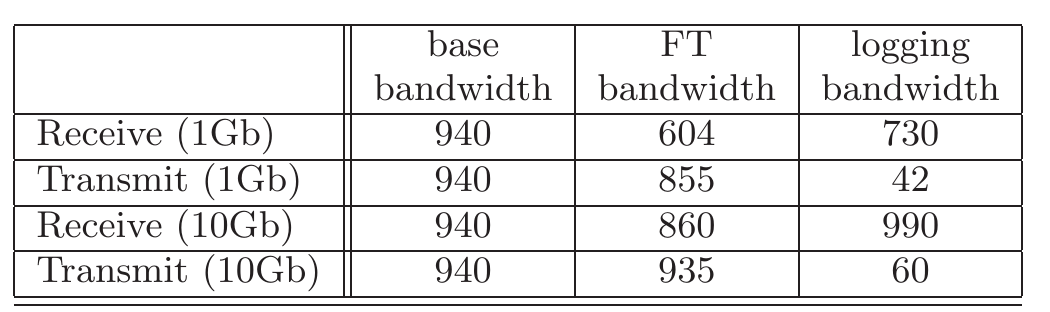
\includegraphics[width=\columnwidth]{figures/original/table-2-network-performance.png}
    \caption{网络发送和接收性能。}
  \end{table}}

\begin{document}
\ifXeTeX
  \CJKsetecglue{}
  \xeCJKsetup{CJKglue={\hskip 0pt plus 0.035em}, CJKecglue={\hskip 0pt}}
\fi
\maketitle
\ifXeTeX
  \CJKsetecglue{}
  \xeCJKsetup{CJKglue={\hskip 0pt plus 0.035em}, CJKecglue={\hskip 0pt}}
\fi

\section*{摘要}

我们实现了一个商用企业级系统，用来提供可容错(fault-tolerant)的VM，%
它的原理是利用另一台服务器上的backup VM来复制primary VM的执行。%
我们在VMware vSphere 4.0中设计了一个完整且易于使用的系统，%
可以运行在通用服务器上，并且通常使真实应用的性能下降不到10\%。此外%
对于一些真实应用，保持primary和backup的lockstep执行\emph{(译者注：
lockstep可以简单理解为“步调一致”，VM-FT是复制状态机，在一定程度上保持
两个VM步调一致、状态同步)}%
所需的数据带宽低于20Mbit/s，这使得在更远距离上实现容错成为可能。%
一个易用的商用系统如果要在failure后自动恢复冗%
余，除了复制VM执行之外，还需要许多额外组件。我们设计并实现了这些额外组件，%
并解决了支持运行企业应用的VM时遇到的许多实际问题。本文将描述我们的基本设计，%
讨论可选设计方案和实现细节，并给出微基准测试和真实应用的性能结果。

\section{引言}

实现可容错服务器的一种常见方法是primary/backup方法[1]，%
也就是始终准备一台backup服务器，在primary服务器故障(fail)时接管(take over)。%
backup服务器的状态必须始终与primary服务器几乎完全一致，%
这样当primary服务器failure时，backup服务器才能立即take over，%
并且以一种对外部客户端隐藏failure且不丢失数据的方式take over。%
复制backup服务器状态的一种方法，是几乎连续地把primary服务%
器所有状态的变化，包括CPU、内存和I/O设备的变化，%
都发送到backup服务器。然而，发送这些状态所需的带宽，%
尤其是内存变化所需的带宽，可能非常大。\emph{(译者注：这种方式被%
称为状态同步，常见的做法是先全量同步，后续同步“增量状态”，也就是上文
提到的“状态变化”)}%

另一种复制服务器的方法有时被称为状态机(state-machine)方法[13]，%
它可以使用少得多的带宽。其思想是把服务器建模为%
deterministic state-machine：让它们从相同的初始状态开始，%
并确保它们以相同顺序接收相同的输入请求，从而保持同步\emph{(译者注：%
这个思路就是复制状态机：给相同的初始态输入相同的操作，得出的%
结果一样，有点机械决定论那味了)}。%
由于大多数服务器或服务都有一些non-deterministic operation，%
\emph{(译者注：假设你有两台机器，都是单核心，同样的硬件配置，核心跑的同%
样的程序，然而它们也可能有不同的“输出”。我举个例子，你的代码里有“时间相关”%
的操作，比如读取CPU时钟，或者应用程序会读取gettimeofday，这样%
即使两个机器配置一样且同时开始运行，也会让“时间敏感”的程序输出不同；%
此外，在操作系统中，随机数也是这样，它实际上综合了来自操作系统的%
各类“混沌的信息”，这类混沌信息也许一部分来自“时间”，因此也会有不确定性)}%
因此必须使用额外的协调机制，确保primary服务器和backup服务器保持同步%
。不过，使primary服务器和backup服务器保持同步所需的额外信息量，%
远小于primary服务器中正在变化的状态量(主要是内存更新)。%

实现协调机制来确保物理服务器的deterministic execution%
[14]是困难的，尤其是在处理器频率不断提高时。相比之下，%
运行在hypervisor之上的VM是实现state-machine方法的极好平台。%
VM可以被视为一个定义良好的state-machine，%
其操作就是被虚拟化机器(包括所有设备)的操作。与物理服务器一样，%
VM也有一些non-deterministic operation(例如读取日时钟%
，或interrupt投递\emph{(译者注：对于两台机器，interrupt投递%
必须完全由primary控制时序，如果任由两台机器执行自己的中断，那么%
会由于中断插入的位置不同导致状态分岔。常见的请求就是两个机器，设置了10ms的时间中断，%
后续运行相同的代码，最后可能因为物理因素，比如芯片频率导致中断插入的位置不一样，%
进而使状态不一致，执行流分岔)}，因此必须向backup VM发送额外信息，%
确保它保持同步。由于hypervisor完全控制VM的执行，包括所有输入的投递，%
因此hypervisor能够捕获primary VM上%
non-deterministic operation的全部必要信息，%
并在backup VM上正确replay这些操作。%
\\\emph{译者注：hypervisor技术可以理解为将硬件拆分给多个虚拟机%
使用，虽然主板上只有一套物理硬件，但是可以依靠“多路复用”的思路实现拆分。%
我们可以选择直接在机器上部署裸金属hypervisor(不依赖于操作系统)。%
读者可以把这种裸金属hypervisor理解为一个用于管理VM虚拟化的简易操作系统，%
在裸机安装这个“微操作系统”后，可以配置它的网络(IP、Mask、Gateway，DNS)，%
外界可以直接进入它的Web UI进行管理，并且它提供了RESTful的API可以创建/销毁/%
暂停/快照虚拟机等功能，直接供外界调用，管理该机器的虚拟机资源。%
\\实际上本文所述的FT系统，需要的主要不是“虚拟化将硬件多路复用”的能力，
而是利用Hypervisor对VM执行边界的控制能力：截获输入、非确定性事件、虚拟中断、%
外部输出，并让backup按相同轨迹重放。实现这些能力需要修改%
hypervisor代码。}%

因此，state-machine方法可以在通用硬件上的VM中实现，不需要修改硬件，%
从而可以立即为最新的微处理器实现fault tolerance。此外，%
state-machine方法所需的低带宽，%
使primary和backup主机在物理上相隔更远成为可能。例如，%
backup VM可以运行在分布于一个园区内的物理机器上，这比运行在同一栋楼%
有更高的可靠性。%

我们在VMware vSphere 4.0平台上使用primary/backup方法%
实现了fault-tolerant VM。该平台以高效方式运行完全虚拟化的%
x86 VM。由于VMware vSphere实现了完整的%
x86 VM，我们能够自动为任何x86操作系统和应用提%
供fault tolerance能力。使我们能够记录primary VM的执%
行并确保backup VM完全相同执行的基础技术称为deterministic replay%
[15]。VMware vSphere Fault Tolerance(%
FT)基于deterministic replay，但增加了构建完整fault tolerance%
系统所需的额外协议和功能\emph{(译者注：后续会介绍为了对外表现为%
“未出现故障切换”，看起来具有输出一致性而设计的\textbf{Output Rule}；%
以及VM FT检测故障的方法；还有为了防止脑裂采取的额外措施；还有后面复杂的%
网络/磁盘IO故障切换后的一致性问题如何解决。所有的这些都需要进行讨论)}。%
除了提供硬件fault tolerance之外，%
我们的系统还会在failure后自动恢复冗余：%
它会在本地cluster中任意可用服务器上启动一个新的backup VM。目前，%
deterministic replay和VMware FT的生产版本都只支持单处理%
器VM。记录-重放多核VM的执行过程的版本仍处于开发阶段，%
它存在严重的性能问题，因为几乎每次对共享内存的访问都可能是不确定的。%

Bressoud和Schneider[3]描述了一个面向HP PA-RISC平台的%
fault-tolerant VM原型实现。我们的方法与之类似，%
但出于性能原因做出了一些根本改变，并考察了多种设计替代方案。此外，%
为了构建一个高效且可供运行企业应用的客户使用的完整系统，%
我们还必须设计并实现系统中的许多额外组件，并处理大量实际问题。%
与讨论过的大多数其他实际系统类似，我们只尝试处理fail-stop failure%
[12]，也就是那些能够在failed服务器造成错误的外部可见行为之前被检测到的%
服务器failure。%
\\\emph{译者注：fail-stop可以是机器简单地直接宕机，也可以是机器尚未%
立刻掉电、内部状态不明，但已经不再对外产生可观察输出。%
对于很多服务器程序来说，客户端只能通过网络观察服务器行为；%
在这一前提下，如果系统能够保证某一时刻之后该服务器不再向外%
发送网络报文、不再响应客户端请求，那么从客户端视角看，它就%
可以被抽象为一种合理的fail-stop故障。(不过，后续读者会%
看到，如果该服务器还能继续写共享存储、访问外部设备或产生其他
外部副作用，仅仅“不发网络包”还不够安全)}

本文其余部分组织如下。首先，我们描述基本设计，并详细说明我们的基础协议，%
这些协议确保在backup VM于primary VM failure后take over%
时不会丢失数据。然后，我们会详细描述为构建一个健壮、完整、%
自动化的系统，我们所必须解决的许多实际问题。我们还描述实现%
fault-tolerant VM时出现的若干设计选择，并讨论这些选择中的权衡。%

接下来，我们给出我们的实现针对若干benchmark和真实企业应用的性能结果。%

最后，我们描述相关工作并作总结。

\section{基本FT设计}

\insertfigureone

Figure 1展示了我们用于fault-tolerant VM的系统基本设置。%
对于一个希望提供fault tolerance能力的VM(被称为primary VM)，%
我们会在另一台物理服务器上运行一个backup VM，使它保持同步，%
并以与primary VM完全相同的方式执行，只是有很小的时间滞后。%
我们称这两个VM处于virtual lockstep\emph{(译者认为可以称为%
“步调一致”)}状态。VM的virtual disk位于%
shared storage上(例如Fibre Channel或iSCSI disk %
array)，因此primary VM和backup VM都可以访问这些磁盘以进行输%
入和输出(我们将在section 4.1讨论一种primary VM和backup VM使用独%
立的非共享virtual disk的设计)。只有primary VM会在网络上宣告自%
己的存在，因此所有network input\emph{(译者注：网络报文)}都%
会到达primary VM。类似地，所有其他输入(例如键盘和鼠标)也只%
会到达primary VM。\emph{(译者注：如果通过VNC连接VM内的Linux%
那么键盘和鼠标也算network input；当然vSphere Web Console/VMRC的控制台%
会直接向VM的虚拟键盘/鼠标设备注入事件，因此确实存在%
keyboard/mouse input。VMware官方资料也明确讨论了Web Console%
和VMRC中的键鼠事件。读者可以暂时不感知keyboard/mouse，就假设咱们%
只能VNC，通篇论文只关注网络和磁盘相关即可)}%

primary VM收到的所有输入都会通过一条称为\textbf{logging channel}的%
网络连接发送给backup VM。%
对于服务器的工作负载而言，主要的输入流量来自网络和磁盘。如下文section 2.1所述，%
为了确保backup VM与primary VM以相同的方式执行%
non-deterministic operation，必要时还会传输额外信息
\emph{(译者注：这里的关键是，backup VM%
不能让自己所在物理机上的外部事件直接决定guest-visible execution。%
比如backup host自己产生的物理timer interrupt、自己收到的外部网络包，%
都不能直接作为backup guest OS的输入。对于guest-visible的timer interrupt、%
I/O completion interrupt、网络输入、磁盘读结果等，primary会记录相关%
log entry，并通过logging channel发送给backup。backup在replay时按照%
log entry指定的内容和执行位置插入这些输入或异步事件，从而消除状态偏移。%
在默认设计中，disk read结果也作为输入由primary通过logging channel发送给backup；%
论文后文还讨论了一种让backup自己执行disk read的替代设计)}。%
结果是，backup VM始终以与primary VM完全相同的方式执行。%

不过，backup VM的输出会被hypervisor丢弃，%
因此只有primary VM会产生实际输出并返回给客户端。如section 2.2所述，%
primary VM和backup VM遵循一个特定协议，其中包括backup VM的%
显式acknowledgment，以确保primary VM failure时不会丢%
失数据。%
\\\emph{译者注：“丢数据”指的是primary已经对外产生了某个可见结果，%
但backup没有收到足够的log来重放到这个结果对应的状态。}%

为了检测primary VM或backup VM是否已经发生故障，我们的%
系统结合使用了两种机制：相关服务器之间的心跳检测，以及%
对logging channel上流量的监控。除此之外，即使出现%
primary服务器和backup彼此失去通信的这种split-brain(脑裂)情况%
\emph{(这里的split-brain不是指系统真的产生了两个合法primary，%
而是指primary和backup所在服务器之间失去通信后，backup可能误判%
primary已经故障并尝试go live；但primary可能其实仍在运行并继续%
对外服务。如果此时backup也开始对外输出，就会出现两个VM同时对外服%
务，导致网络响应、磁盘写入和客户端状态混乱)}，%
我们也必须确保primary VM和backup VM中只有一个会接管执行%
\emph{(译者注：后文会说明，这里利用了共享磁盘上的test-and-set操作)}。%

在下面各节中，我们将对几个重要方面给出更多细节。在section 2.1，%
我们给出deterministic replay技术的一些细节，%
该技术通过logging channel发送的信息确保primary VM和%
backup VM保持同步。在section 2.2，我们描述FT协议的一条基本规则，%
它确保primary VM failure时不会丢失数据。在section 2.3，%
我们描述用于以正确方式检测并响应failure的方法。

\subsection{deterministic replay的实现}

如前所述，复制服务器(或VM)的执行可以被建模为复制一个%
deterministic state-machine。如果两个%
deterministic state-machine从相同的初始状态开始，%
并以相同顺序获得完全相同的输入，那么它们将经历相同的状态序列，并产生相同的输出。%
VM具有广泛的input集合，包括传入的network packet、disk read，
以及来自键盘和鼠标的input。%
non-deterministic event(例如virtual interrupt)%
和non-deterministic operation(例如%
读取处理器的时钟周期计数器)也会影响VM的状态。%
由于VM可能运行任意操作系统和任意工作负载\emph{(译者注：不能假定VM只运行%
类似“纯计算”的任务，也得考虑是否会读取系统时间，或者进行某些依赖系统%
时间片的工作。实际上network就是这样的工作，TCP协议其实内部会依赖定时器)}，%
这为VM的执行带来了三个挑战：(1)正确捕获保证%
backup VM deterministic execution所需的所有输入和%
non-determinism；(2)正确地把这些输入和%
non-determinism应用到backup VM；(3)%
以不降低性能的方式做到这一点。此外，x86微处理器中的许多复杂操作%
具有未定义的、因而也是non-deterministic的副作用。%
捕获这些未定义副作用并replay它们以产生相同状态，是另一个挑战。%
\\\emph{%
译者注：这里的disk read是从外部磁盘向VM引入数据的操作。guest OS driver%
通常会在guest memory中的descriptor中描述请求，再通过MMIO doorbell通知%
虚拟设备；具体队列布局因设备模型而异。对于read，设备或hypervisor取得磁盘%
数据后，会在确定的completion投递点更新guest memory和虚拟设备状态，再向%
guest注入completion interrupt。VMware FT需要记录read数据、completion结果%
及其精确投递位置，使backup在相同执行点看到相同结果。guest在completion之前%
访问目标内存仍可能看到旧数据，这正是section 3.4使用bounce buffer隔离异步%
DMA更新的原因。对于write，数据从guest memory流向磁盘，属于external output；%
其completion状态和投递时机仍可能具有non-determinism，也需要记录必要信息。}%

VMware deterministic replay[15]正是为VMware %
vSphere平台上的x86 VM提供了这种功能。%
deterministic replay会把VM的输入以及与VM执行相关的所有可能%
的non-determinism，record为一串log entry并写入log %
file。之后通过读取文件中的log entry，可以精确replay VM的执行。%
对于non-deterministic operation，%
会记录足够的信息，使该操作能够以相同的状态变化和输出被复现。%
对于timer interrupt或IO完成interrupt等%
non-determinism事件，还会record事件发生时的精确指令。%
在replay期间，该事件会在指令流中的同一位置被投递。%
VMware deterministic replay实现了一种高效的事件%
record和事件投递机制，采用了多种技术，包括与AMD[2]和Intel[8]%
共同开发的硬件性能计数器\emph{(译者注：硬件性能计数器是用%
来分析性能的，它里面有很多事件可以使用，但要实现VM FT只需关注%
instructions retired就行，它代表已提交的机器指令数)}。%

Bressoud和Schneider[3]提到把VM的执行划分为若干epoch，%
诸如interrupt这样的non-deterministic event只在一个%
epoch结束时投递。epoch的概念似乎被用作一种批处理机制，%
因为在事件发生的精确指令处分别投递每个interrupt成本太高。然而，%
我们的事件投递机制足够高效，因此VMware deterministic replay%
不需要使用epoch。每个interrupt都会在发生时被记录，%
并在replay时高效地投递到适当的指令处。
\\\emph{译者注：先简要描述Bressoud和Schneider的epoch机制。%
该系统同样采用primary/backup架构，两台机器上都有一种特殊寄存器，%
该寄存器会在每执行完一条指令后递减一次；当其变为负数时，%
处理器会触发一个控制中断，使hypervisor重新获得控制权。%
例如，如果将该寄存器设置为1000，那么按照字面语义，VM会在%
执行完1001条指令后结束当前epoch，并陷入由该特殊寄存器触发的%
控制中断(hypervisor层的中断)。此时hypervisor可以统一处理本epoch内缓存起来的%
普通VM中断。这里的普通VM中断，是指timer interrupt、I/O完成%
interrupt、network interrupt等guest OS正常运行时会看到的中断，%
它们不同于用于结束epoch的控制中断。%
\\对于primary和backup来说，它们从相同状态启动，并且各自的%
hypervisor都会将该特殊寄存器设置为相同的值，例如1000。%
在一个epoch内，primary收到的普通VM中断不会立即投递给%
primary VM，而是先由primary hypervisor记录并缓存起来；%
backup本机收到的普通VM中断也不会直接投递给backup VM，%
而是由backup hypervisor丢弃。%
primary VM和backup VM会执行对应的epoch，但backup至少落后primary%
一个epoch。当primary的epoch结束时，primary hypervisor把本epoch内%
缓存的普通VM中断列表发送给backup，并等待ack。backup执行到对应epoch%
边界后，等待并接收该中断列表，先向primary返回ack，再向backup VM投递%
同一批中断。primary收到ack后，才在自己的epoch边界向primary VM投递%
这批中断；随后双方分别进入下一个对应的epoch。}%

\subsection{FT协议}

\insertfiguretwo

对于VMware FT，我们使用deterministic replay来生成必要的日志条目，%
用来记录primary VM的执行过程。%
但我们不是把这些log entry写入磁盘，而是通过logging channel把%
它们发送给backup VM。%
backup VM会实时replay这些log entry，%
因此以与primary VM完全相同的方式执行。不过，为了确保真正实现fault %
tolerance，我们必须在logging channel上的log entry之%
外增加严格的FT协议。我们的基本要求如下：%

\begin{quote}
\noindent\textbf{Output Requirement:}如果backup VM在primary VM %
failure后take over，那么backup VM将继续以一种完全符合%
primary VM已经发送到外部世界的所有输出的方式执行。%
\end{quote}

\noindent{}注意，在发生failover之后(也就是backup VM在primary VM %
failure后take over之后)，由于执行过程中会发生许多%
non-deterministic event，backup VM很可能开始以一种与%
primary VM原本继续执行时非常不同的方式执行。%
不过，只要backup VM满足\textbf{Output Requirement}，%
在failover到backup VM的过程中就不会丢失任何外部可见的状态或数据，%
客户端也不会察觉服务中断或不一致。%

\textbf{Output Requirement}可以通过delay任何外部输出%
(通常是一个网络包)来保证，直到backup VM已经接收到所有%
必要信息，使其能够至少将执行重放到该输出操作发生的位置。%
一个必要条件是，backup VM必须已经接收到该输出操作之前生%
成的所有日志条目。这些日志条目将使它能够执行到最后一个日志%
条目所在的位置。然而，假设primary VM在执行完输出操作后立即发生%
故障，backup VM就必须知道自己必须继续replay，直到该输出操%
作的位置，并且\textbf{只能在那个位置“上线”}(也就是停止重放，并接%
管成为primary VM，见section 2.3)。如果备份虚拟机在输出操作之%
前的最后一个日志条目处就上线(go live)，那么某些non-deterministic event%
(例如传递给VM的timer interrupt)可能会在它执行该输出%
操作之前改变它的执行路径。
\\\emph{
译者注：具体来说，常见log entry包括：
\begin{enumerate}
  \item \textbf{input event log}：记录外部输入及其投递位置，例如incoming network packet、
  disk read completion、键盘输入、鼠标输入等。这类事件不仅表现为interrupt，
  还会把外部数据带入VM，因此必须记录数据内容和投递位置。
  \item \textbf{interrupt/event log}：记录不携带外部数据、但会改变guest执行路径的
  non-deterministic event，例如timer interrupt、disk write completion interrupt、
  以及其他设备completion interrupt。这类事件的重点是记录它在指令流中的精确投递位置。
  \item \textbf{non-deterministic instruction log}：记录某些非确定性指令或特殊读操作的结果，
  例如读取时间戳计数器、时钟、某些设备状态寄存器等。如果guest执行这类操作时得到的结果
  不能由初始状态和普通指令流确定，那么replay时也必须使用primary记录下来的结果。
  \item \textbf{output log entry}：记录external output operation在指令流中的发生位置，
  例如network packet send，必要时也包括某些对外可见的磁盘写操作。它的核心作用不是让
  backup在replay时再次对外输出，而是把output point归一化为log stream中的一个
  marker，使backup知道自己必须至少replay到这个位置，才能安全go live。
\end{enumerate}
}

在上述约束下，强制执行\textbf{Output Requirement}最简单的方法，%
是在每个output operation处创建一个特殊的log entry。于是，%
\textbf{Output Requirement}可以通过下面这条具体规则来强制执行：%

\begin{quote}
\noindent\textbf{Output Rule:}在backup VM收到并acknowledge与产生该%
output的操作相关联的log entry之前，primary VM不得向外部世界发送该输出%
(向外部世界发送输出包括网络packet输出和磁盘操作)。%
\end{quote}

如果backup VM已经收到所有log entry，包括产生输出的操作对应的log %
entry，那么backup VM就能够精确复现primary VM在该输出点处的状%
态；因此，如果primary VM死亡，backup VM将正确到达一个与该输出一致%
的状态。相反，如果backup VM在没有收到所有必要log entry的情况下%
take over，那么它的状态可能很快发散，导致与primary VM的输出不一致%
。\textbf{Output Rule}在某种程度上类似于[11]中描述的方法，%
其中“外部同步”的IO实际上可以被缓冲，只要它在下一次外部通信之前确实写入磁盘即%
可。%

注意，\textbf{Output Rule}并没有要求停止primary VM的执行。%
我们只需要delay发送输出，而VM本身可以继续执行\emph{(译者注：
这也是为什么这个系统能较少地影响机器性能的部分原因，不会像之前提%
到的epoch系统影响到primary正常运行)}。由于操作系统使用非阻塞的网%
络和磁盘输出，并通过异步interrupt表示完成，VM可以很容易继续执行，%
并且不一定会立即受到输出delay的影响。相比之下，以前的工作[3, 9]通常指%
出，primary VM在执行输出之前必须完全停止，直到backup VM %
acknowledge已收到来自primary VM的所有必要信息。\emph{
(译者注：比如前面的epoch，primary和backup都会停在执行完某个epoch
之后，然后这里会暂停primary VM，等到交互完成后双方才能继续执行。
因此这个系统虽然是“批处理”思想的系统，但也是性能损失较大的)}%

作为示例，我们在Figure 2中展示了一张说明FT协议要求的图。该图展示了%
primary VM和backup VM上事件的时间线。从primary VM线指向%
backup VM线的箭头表示log entry的传输，从backup VM线指向%
primary VM线的箭头表示acknowledgment。异步事件、%
输入和output operation的信息都必须作为log entry发送到%
backup VM，并得到acknowledgment。如图所示，%
到外部世界的输出会被delay，直到primary VM收到backup VM的%
acknowledgment，表明backup VM已经收到与该output %
operation相关联的log entry。%
只要遵循Output Rule，backup VM就能够以一种与primary VM最%
后一次输出一致的状态take over。%

我们无法保证在failover场景中所有输出都恰好产生一次。%
如果在primary VM打算发送输出时不使用带two-phase commit的%
transaction，backup VM就无法判断primary VM是在发送最后%
一个输出之前还是之后崩溃。幸运的是，network infrastructure(%
包括TCP的常见使用方式)本来就是为了处理丢失包和相同的(重复)包而设计的。%
注意，primary VM的传入包也可能在primary VM failure期间丢失%
，因此不会被投递到backup VM。不过，传入包可能因为许多与服务器%
failure无关的原因被丢弃，因此network infrastructure、%
操作系统和应用都被编写成能够补偿丢包。%
\\\emph{译者注：
\\这里并不能保证packet恰好发送一次。primary可能在最后一个packet%
真正发出之前或之后failure，因此客户端可能观察到丢包或一个包。%
backup决定上任后会切断log channel，然后重放log entry，%
对于发送网络报文的log entry直接忽略，因此这可能丢包，或者发出一个包；
当然重放发送网络报文的log entry时重新发包也是正确的实现，在这种实现中，%
真实发出一个包或者两个包都是有可能的。无论是哪种实现，都是正确的。%
\\\\Output Rule保证的是：只要某个输出已经对外可见，backup就拥有足够的%
log，可以在failover后到达与该输出一致的状态。TCP等网络协议本来就会%
处理丢包、重复和乱序，因此FT层不需要判断最后一个packet究竟是否发出。%
相比于本文主要描述的共享磁盘(它本质上也是一种输出设备)，%
这种磁盘I/O没有上述网络协议的语义，需要额外考虑和处理，相关处理见section 3.4。}%

\subsection{检测并响应failure}

如上所述，如果另一个VM看起来已经failure\emph{(primary%
和backup都需要感知对方，对面挂了就采取一定措施)}，primary VM和%
backup VM必须快速响应。如果backup VM failure，%
primary VM将go live，也就是离开recording mode(因此停止%
在logging channel上发送log entry)并开始正常执行%
\emph{(译者注：实际上这里说primary go live用词不妥，它的意思%
仅仅是退出recording模式，变成独立运行/不受保护的模式，%
并不代表之前就不是“live”的，它仅仅是说后续不再需要得到backup的ack确认后%
才能对外输出，而是放弃容错，确保至少能对外提供服务)}。%
如果primary VM failure，backup VM也应类似地go live，%
但这个过程稍微复杂一些。由于backup VM的执行存在滞后，%
它很可能已经接收并acknowledge了若干log entry，%
但由于尚未到达执行中的相应位置，这些log entry还没有被消费而被%
堆积。backup VM须继续执行并消费日志，直到最后一条log entry被重放%
\emph{(译者注：log entry类型众多，读者可以去2.2的译者注查阅)}，%
此时，backup VM将停止replay模式，并开始作为普通VM执行。%
本质上，backup VM已被提升为primary VM(但此时它缺少一个backup VM)。%
由于它不再是backup VM，新的primary VM现在会在guest OS执行%
output operation时向外部世界产生输出。在切换到正常模式期间，%
可能需要进行一些设备相关的操作，才能使这些输出正确发生。特别是对于网络，%
VMware FT会自动在网络上宣告新primary VM的MAC地址，%
使物理网络交换机知道新primary VM位于哪台服务器\emph{(%
译者注：这样后续来自客户端的网络报文才能继续被处理)}。此外，%
新提升的primary VM可能需要重新发出一些磁盘IO(如section 3.4所述)。%

尝试检测primary VM和backup VM failure的方法有很多。%
VMware FT使用运行fault-tolerant VM的服务器之间的UDP %
heartbeat来检测某台服务器是否可能已经崩溃。此外，%
VMware FT会监控从primary VM发送到backup VM的logging %
traffic，以及从backup VM发送到primary VM的%
acknowledgment。由于有定期的timer interrupt，%
对于正常运行的guest OS，logging traffic应当是规律的，%
且不会停止。因此，log entry或acknowledgment的流动停止可能表%
明某个VM发生failure。如果heartbeat或logging %
traffic停止超过某个特定超时时间(大约几秒)，就会宣布发生failure。%

然而，任何这样的failure detection方法都容易受到%
split-brain问题的影响。如果backup服务器停止接收来自primary%
服务器的heartbeat，这可能表示primary服务器已经failure，%
也可能只是表示仍在正常运行的服务器之间失去了所有网络连通性%
\emph{(译者注：也就是backup和primary发生分区，互相无法ping%
到对方，UDP的heartbeat心跳包也发不过去，都认为对方死亡)}。%
如果此时backup VM go live，而primary VM实际上仍在运行，%
那么很可能发生数据损坏，并给与VM通信的客户端带来问题。因此，%
当检测到failure时，我们必须确保primary VM和backup VM中只有%
一个go live。为了避免split-brain问题，我们利用存储VM %
virtual disk的shared storage。当primary VM或%
backup VM想要go live时，它会在shared storage上执行一个%
atomic的test-and-set操作。如果操作成功，该VM就被允许go live%
。如果操作失败，那么另一个VM一定已经go live，因此当前VM实际上会停止自身%
(“自杀”)。如果VM在尝试执行该atomic操作时无法访问shared %
storage，那么它只会等待，直到可以访问为止。注意，%
如果shared storage由于存储网络中的某种failure而不可访问，%
那么该VM很可能无论如何都无法做有用工作，因为virtual disk位于同一个%
shared storage上。因此，使用shared storage解决%
split-brain情况不会引入额外的不可用性。%
\\\emph{译者注：论文中的shared storage不是由guest OS%
直接访问的网络盘，也不是挂载在guest OS文件系统层中的%
对象。你可以把它简单理解为仅能在hypervisor层使用的%
共享块存储，它的接口很简单，只有Read(offset, length)%
和Write(offset, data)，看起来就是一块大的共享数组。%
hypervisor再把这个共享存储模拟成一个真正的磁盘设备，guest OS%
感知到的仍然是/dev/sda这样的本地块设备。%
\\\\当操作系统尝试提交IO请求的时候，会向ring放置IO Req，%
然后idx++，写入MMIO。VM会截获这个MMIO写入事件然后VM-Exit让%
VM获得控制权，此时它就会把guest OS的磁盘IO Req转换为共享存储%
读写。此外，test-and-set操作也是在hypervisor层进行的，%
guest OS无感知。}%

设计的最后一个方面是，一旦发生failure并且其中一个VM已经go live，%
VMware FT会通过在另一台host上启动新的backup VM来自动恢复冗余。%
虽然大多数先前工作没有覆盖这个过程，但它对于使fault-tolerant VM真%
正有用是根本性的，并且需要仔细设计。更多细节见section 3.1。

\section{FT的实际实现}

section 2描述了FT的基本设计和协议。然而，要创建一个可用、健壮且自动化的系统，%
还必须设计并实现许多其他组件。

\subsection{启动和重启FT VM}

必须设计的最大额外组件之一，是一种能够以与primary VM%
相同状态启动backup VM的机制。这个机制也会在发生failure%
之后重新启动backup VM时使用。因此，该机制必须能够用于一个%
处于任意状态的正在运行的primary VM(也就是说，并不只是用于%
启动阶段)。此外，我们希望该机制不会显著干扰primary VM的执%
行，因为这会影响该VM当前的任何客户端。%

对于VMware FT，我们改造了VMware vSphere现有的VMotion功%
能。VMware VMotion[10]允许把一个正在运行的VM从一台服务器迁移到%
另一台服务器，并且造成的干扰很小，VM暂停时间通常小于一秒。%
我们创建了一种修改后的VMotion，它会在远程服务器上创建一个VM的精确运行副%
本，但不会销毁本地服务器上的VM。也就是说，我们修改后的FT VMotion会把一%
个VM克隆到远程host，而不是迁移它。FT VMotion还会建立logging %
channel，并使源VM以primary VM身份进入recording mode%
，使目标VM以新backup VM身份进入replay mode。%
与普通VMotion一样，FT VMotion通常使primary VM的执行暂停%
不到一秒。因此，在一个正在运行的VM上启用FT是一个简单且非破%
坏性的操作。%
\\\emph{译者注：
老式操作系统可能主要依赖timer interrupt来推进系统时间。例如，%
硬件每10ms产生一次定时器中断，那么内核收到10次中断后，就认为大约%
过去了100ms。现代操作系统通常不会仅靠这种周期性tick来计算当前时%
间，而是会选择某个clocksource，例如x86机器上的TSC%
(Time Stamp Counter，CPU时间戳计数器)，或者虚拟化环境中的%
paravirtual clock。调用gettimeofday时，系统会读取当前%
clocksource的计数值，与内核timekeeper中保存的基准计数值%
(如cycle\_last)相减，将cycle差值换算成纳秒，再加到内核维%
的wallclock基准时间上，最后返回给用户态。很多系统还会通过%
vDSO在用户态完成这一步，避免每次都陷入内核。
\\针对VM暂停和迁移，读者可能会问：在复制期间，如果VM大约暂停了1s，%
是否会导致VM内部读到的时间落后现实世界时间(wallclock)1s？可%
以这样理解：如果系统真的完全依赖timer interrupt计数来推进时间，%
并且暂停期间没有收到这些中断，那么恢复后确实可能出现时间落后；但现%
代虚拟化环境通常不会简单依赖补发timer interrupt来追赶时间。%
hypervisor可以通过虚拟化TSC、虚拟时钟偏移、paravirtual clock%
或时间同步机制，让guest OS在下一次读取clocksource或调用%
gettimeofday时看到已经校正后的wallclock(real world clock)。%
因此，VM暂停1s后，不需要向guest OS连续注入大量timer interrupt来弥补这1s。%
wallclock的推进和timer interrupt的注入是两个不同层面的问题；VM恢复时，%
hypervisor会根据虚拟定时器的类型和语义处理已经过期的timer，可能合并或投递%
timer interrupt，并不保证固定补发一个中断。
\\\\读取wallclock也是一种non-deterministic operation。原因是wallclock
来自VM外部，如果primary VM和backup VM分别读取各自host的真实时间，
它们可能得到不同结果，从而导致执行路径分叉。VM FT的做法是：primary VM
执行这类读取操作时，由hypervisor返回一个虚拟时间值，并把该返回值及其发生位置
写入replay log；backup VM replay到同一位置时，不读取自己的真实时间，而是直接
使用log中记录的值。这样，primary和backup看到的时间完全一致。
需要注意的是，用户态的gettimeofday不一定每次都会直接产生log entry。
如果它只是读取guest memory中由guest OS维护的时间变量，那么这个普通内存读取
本身是确定性的。真正需要记录的是把外部时间引入VM的边界操作，例如读取虚拟时钟
设备、执行RDTSC，或者timer interrupt推进guest OS时间状态。}%

启动backup VM的另一个方面，是选择在哪台服务器上运行它。%
fault-tolerant VM运行在能够访问shared storage的服务器cluster中，%
因此所有VM通常都可以在cluster中的任意服务器上运行。%
这种灵活性使VMware vSphere即使在一台或多台服务器已经failure时%
，也能恢复FT冗余。VMware vSphere实现了一个维护管理和资源信息的%
cluster服务。当发生failure并且某个primary VM现在需要一个新%
的backup VM来重新建立冗余时，primary VM会通知clustering service%
它需要一个新的backup。clustering service根据资源使用%
情况和其他约束确定运行backup VM的最佳服务器，并调用FT VMotion来创%
建新的backup VM。结果是，VMware FT通常能够在服务器failure后%
的几分钟内重新建立VM冗余，并且整个过程不会对fault-tolerant VM的%
执行造成任何可察觉的interrupt。

\subsection{管理logging channel}

\insertfigurethree

管理logging channel上的流量涉及一些有趣的实现细节。在我们的实现中，%
hypervisor为primary VM和backup VM维护一个大的log %
entry缓冲区。当primary VM执行时，它会把log entry生成到log %
buffer中；类似地，backup VM会从自己的log buffer消费log %
entry。primary VM log buffer的内容会尽快刷新到logging %
channel，log entry也会在到达后尽快从logging channel读%
入backup VM的log buffer。backup VM每次从网络读入一些log %
entry到自己的log buffer时，都会向primary VM发送%
acknowledgment。这些acknowledgment使VMware FT%
能够确定那些被\textbf{Output Rule} delay的输出何时可以发送。%
Figure 3展示了这一过程。\\\emph{译者注：log entry包含，%
timer/disk-write-completion interrupt、wallclock read、%
鼠标/键盘/network/disk-read-completion input，以及为了满足%
\textbf{Output Rule}的output log entry，这些output包括%
写共享磁盘、写外部设备，还有对外写网络报文。}%

如果backup VM在需要读取下一条log entry时遇到空的log buffer%
，它会停止执行，直到有新的log entry可用\emph{(译者注：%
backup已经没有下一条%
log entry可读，因此它不知道primary接下来是否会在某个精确指%
令位置收到interrupt、disk completion、timer interrupt%
等非确定性事件。即使backup接下来执行的普通指令本身是确定性的，%
它也不能擅自继续执行，因为下一条非确定性事件可能本应发生在下一条%
或很近的某条指令之后。backup只有在读到下一条log entry后，才知%
道可以安全执行到哪个指令位置，并在该位置注入相同的非确定性事件。%
因此，backup不是“看到确定性代码就能一直跑”，而是“在已知下一条%
log entry边界的前提下，可以连续执行边界之前的确定性指令”。%
当log buffer为空时，这个边界未知，所以必须暂停)}。%
由于backup VM不与外部通信%
，这种暂停不会影响VM的任何客户端。类似地，如果primary VM在需要写入%
log entry时遇到满的log buffer，它必须停止执行，%
直到log entry能够被刷新出去。这种执行停止是一种自然的流控机制，%
会在primary VM过快产生log entry时降低其速度。然而，%
这种暂停可能影响VM的客户端，因为primary VM会完全停止并且无响应，%
直到它能够record log entry并继续执行。因此，%
我们的实现必须被设计成尽量降低primary log buffer被填满的可能性。%
\\\emph{译者注：简化的primary执行与日志生成伪代码；实际实现还包含%
并发的日志发送、ACK处理和buffer回收逻辑：}
\begin{Verbatim}[
  fontsize=\scriptsize,
  breaklines=true,
  breakanywhere=true
]
// VM执行循环
func PrimaryRunLoop(vm *VM) {
    for vm.Running {
        result := RunGuestUntilExitOrEvent(vm)

        switch result.Type {

        case "DETERMINISTIC_EXECUTION":
            // 普通CPU指令、内存读写、guest OS内部逻辑
            // 不写log，backup自己也能执行出来
            continue

        case "NONDETERMINISTIC_EVENT":
            // 例如timer interrupt、network input、disk I/O completion
            entry := LogEntry{
                Seq:        NextSeq(),
                EventType:  result.EventType,
                InstrCount: vm.InstrCount(),
                Payload:    result.Payload,
            }

            // 关键：primary把非确定性事件写入自己的logbuffer
            primaryLogBuffer.Append(entry)

            // 然后才把这个事件注入/交给guest
            InjectEventToGuest(vm, entry)

        case "OUTPUT_OPERATION":
            // guest想对外输出，比如发网络包
            // 注意：output本身可能是deterministic产生的，
            // 但它有外部副作用，所以要遵守OutputRule

            entry := LogEntry{
                Seq:        NextSeq(),
                EventType:  "OUTPUT_MARKER",
                InstrCount: vm.InstrCount(),
                Payload:    nil,
            }

            primaryLogBuffer.Append(entry)

            output := PendingOutput{
                Packet:      result.Packet,
                RequiredSeq: entry.Seq,
            }

            // 不能马上发出去，先放到pending队列
            pendingOutputs.Append(output)

        case "VM_FAIL_OR_STOP":
            return
        }
    }
}
// 一个单独的线程，作为背景线程运行
func HandleBackupAck(ackedSeq uint64) {
    primaryLogBuffer.ReleaseThrough(ackedSeq)

    for pendingOutputs.HasReady(ackedSeq) {
        output := pendingOutputs.PopReady(ackedSeq)
        SendToExternalWorld(output.Packet)
    }
}
\end{Verbatim}
\emph{如果Append因buffer已满而无法继续，primary执行循环就必须等待。%
日志发送循环把entry发送给backup；收到ACK后，ACK处理逻辑回收已确认的%
log entry，并释放满足Output Rule的pending output。}

primary log buffer可能被填满的一个原因，是backup VM执行得太慢，%
因而消费log entry也太慢。一般来说，backup VM必须能够以大致等于%
primary VMrecord执行的速度来replay执行。幸运的是，%
在VMware deterministic replay中，%
record和replay的开销大致相同。然而，如果承载backup VM的服务器%
上运行了许多其他VM(因而资源过度提交)，那么即使backup hypervisor的VM%
调度器尽力调度，backup VM也可能无法获得足够的CPU和内存资源来以%
primary VM的速度执行。
\\\emph{译者注：这里的内存资源不足，并不是说guest OS看到%
的内存容量变小了。创建VM时确实会指定一个内存大小，例如4GB%
或8GB，guest OS也会认为自己拥有这么多“物理内存”。但是这%
只是guest看到的guest physical memory大小，这些guest物理页背%
后仍然需要宿主机(host)真实物理内存承载。如果承载backup VM的机器上%
运行了很多VM，所有VM配置的内存总量可能超过物理机的真实物理内存，%
这就是memory overcommit，也就是内存超卖。此时hypervisor可能%
通过ballooning、memory compression、host swapping、page sharing%
等机制回收或腾挪内存页。如果host物理内存实在不够，hypervisor%
也可能从其他VM回收分配给该VM的物理页；直观地说，这有点像向其他VM%
“借”内存，但不是把另一台VM整体永久暂停后直接搬走它的内存。%
更准确地说，hypervisor可以把其他VM中暂时不用、可回收或者%
优先级较低的页面压缩后放入host内存中的压缩区，或者写入host swap所在的%
磁盘空间，也可以通过ballooning%
让该guest OS主动释放一些页面，再把释放出来的host物理页分配%
给当前更需要资源的VM。被回收页面的VM通常仍然可以继续运行，%
但如果它之后再次访问这些被压缩或换出的页面，就需要等待hypervisor%
重新解压或从swap读回，因此会发生短暂停顿。更底层地说，guest OS%
维护自己的页表，把guest virtual address映射到guest physical address；hypervisor%
还会维护第二级地址映射，例如Intel EPT或AMD NPT，把guest physical%
address映射到host physical address。当某个guest物理页暂时没有映射到host%
物理页时，guest再次访问该页不会由guest OS自己处理，而是触发%
EPT violation或nested page fault，使CPU退出到hypervisor。随后%
hypervisor把该页从swap中读回，或者解压、重新分配host物理页，%
并恢复对应的二级页表映射。这个过程更准确地说是VM-exit，不是%
普通外部中断。它不会改变guest OS看到的内存大小，但会增加内存%
访问延迟。因此backup VM虽然名义上仍拥有创建时配置的内存容量，%
却可能因为host层面的物理内存竞争、换页、向其他VM回收页面，%
或者NUMA局部性变差而replay变慢。}%

除了避免log buffer被填满导致意外暂停之外，我们不希望执行滞后变得太大还有%
另一个原因。如果primary VM failure，backup VM必须通过%
replay它已经acknowledged的所有log entry来“追上来”%
，然后才能go live并开始与外部世界通信。完成replay所需时间基本上就是%
failure发生点的执行滞后时间，因此backup VM go live所需时间大致%
等于failure detection时间加上当前执行滞后时间。因此，%
我们不希望执行滞后时间很大(超过一秒)，因为这会显著增加failover%
(故障接管)的时间。\emph{(译者注：因为backup必须重放完，直到处理完%
最后一条log entry)}%

因此，我们有一个额外机制来降低primary VM的速度，%
防止backup VM落后太多。在发送和acknowledgment log entry%
的协议中，我们会发送额外信息，以确定primary VM和%
backup VM之间的实时执行滞后。通常执行滞后小于100毫秒。%
如果backup VM开始出现显著执行滞后(例如超过1秒)，%
VMware FT会通过通知调度器给primary VM略少一些CPU(开始时只减少%
几个百分点)来减慢primary VM。我们使用一个缓慢的反馈循环，%
逐步找出适合primary VM的CPU限制，使backup VM能够匹配其执行。%
如果backup VM继续落后，我们会继续逐步降低primary VM的CPU限制。%
相反，如果backup VM追上来了，我们会逐步提高primary VM的CPU限制%
，直到backup VM恢复到只有轻微滞后。%
\\\emph{译者注：\textbf{Output Rule}会把对外输出延迟到backup VM ACK对应%
log entry之后。例如logging channel的一次确认往返若耗时约40ms，额外出包%
延迟可能接近这一量级；实际延迟还取决于log flush、批处理和调度。}%

注意，primary VM的这种减速非常少见，通常只会在系统处于极端压力下发生。%
section 5中的所有性能数字都包含了任何这类减速的成本。

\subsection{FT VM上的操作}

另一个实际问题是处理可能应用于primary VM的各种控制操作。例如，%
如果primary VM被显式关机，backup VM也应停止，%
而不应尝试go live。再如，primary VM上的任何resource management%
变化(例如增加CPU份额)也应应用到backup VM。%
对于这类操作，会通过logging channel从primary VM向%
backup VM发送特殊的control entry，以便在backup VM上执行%
相应操作。%

一般来说，对VM的大多数操作都只应在primary VM上发起。%
VMware FT随后会发送必要的control entry，%
使backup VM发生相应变化。唯一可以在primary VM和backup VM上%
独立执行的操作是VMotion。也就是说，primary VM和backup VM可%
以独立地VMotion到其他host。注意，VMware FT会确保两个VM都不会%
被移动到另一个VM所在的服务器上，因为那种情况将不再提供%
fault tolerance能力。%

primary VM的VMotion比普通VMotion增加了一些复杂性，%
因为backup VM必须在适当时刻断开与源primary VM的连接，%
并重新连接到目标primary VM。backup VM的VMotion也有类似问题%
，但还增加了额外复杂性。对于普通VMotion，我们要求在VMotion最终切换%
发生时，所有未完成的磁盘IO都被静止(也就是完成)。对于primary VM，%
通过等待物理IO完成并把这些完成投递给VM，就很容易处理这种静止。然而，%
对于backup VM，没有简单方法能在任何要求的位置使所有IO都完成，%
因为backup VM必须replay primary VM的执行，%
并在相同的执行点完成IO。primary VM可能正在运行一种workload，%
在正常执行期间始终有磁盘IO正在进行。VMware FT有一种独特方法来解决这个问%
题。当backup VM到达VMotion的最终切换点时，%
它会通过logging channel请求primary VM临时静止其所有IO。%
随后，backup VM在replay primary VM的静止操作执行时，%
它自己的IO也会自然地在同一个执行点被静止。
\\\emph{译者注：这是说了两个问题：一是primary从一台host迁移到另外一台；%
二是backup从一台host迁移到另外一台。其中后者更难一点。
\\\\primary迁移可以理解为：在最终切换点暂停primary VM，等待所有in-flight%
磁盘I/O完成，并把这些I/O completion交付进VM的虚拟设备状态/待处理中断状态中，%
从而形成一个没有inflight disk I/O的干净迁移点。随后旧primary停止运行，%
把旧VM状态切换到新host，并且配置网络，新primary从该状态继续执行。%
backup则在正确的log边界断开旧primary，并连接新primary。%
此后新primary继续作为primary记录non-determinism事件，生成log entry，%
并通过新的logging channel发送给backup。%
\\\\backup迁移比primary迁移更麻烦：原因是backup VM并不是自由执行的VM，%
而是在replay primary VM的执行流；因此backup不能为了迁移而任意选择一个时刻%
交付磁盘I/O completion，否则就可能破坏和primary相同的执行轨迹。%
当backup VMotion进入最终切换阶段时，backup会通过logging channel请求primary%
暂时quiesce磁盘I/O。primary执行这个quiescing operation，等待已有in-flight%
磁盘I/O完成，并把completion交付给VM；该操作随后被记录进FT log。backup在%
replay primary执行流时，会在同一个执行点replay到这个quiescing operation，%
于是backup的I/O也自然进入quiesced状态。此时backup才可以安全地完成迁移，%
旧backup停止运行，目标主机上的backup从该状态继续replay primary后续产生的log。}%

\subsection{磁盘IO的实现问题(重要，难点)}

\emph{译者注：此处我解释磁盘IO工作流程。guest OS启动并初始化磁盘驱动时，会在%
guest物理内存中分配Descriptor Table、Available Ring和Used Ring。%
Descriptor Table用于描述请求涉及的内存buffer；Available Ring由guest驱动%
写入、虚拟设备读取，用于发布新请求；Used Ring由虚拟设备写入、guest驱动%
读取，用于返回已经完成的请求。%
\\Descriptor Table中的一个descriptor包含buffer的guest物理地址、长度、%
访问方向以及下一个descriptor的编号。一个磁盘请求不一定只使用一个%
descriptor，而可能由一条descriptor chain组成。例如，一个write请求通常%
包含请求头、待写数据和完成状态三个部分：请求头和待写数据由guest写入、%
设备读取，完成状态则由设备写入、guest读取。guest驱动会记录descriptor %
chain的head ID，以便之后根据该ID找到原始请求。%
\\Available Ring中保存的不是完整IO请求，而是descriptor chain的head ID。%
avail.idx是位于guest物理内存中的16位计数器，由guest驱动维护，%
并不是一个MMIO寄存器。假设avail.idx初始值为0，guest准备提交%
三个分别由descriptor 7、12和4描述的请求，那么guest会依次执行%
avail.ring[0]=7、avail.ring[1]=12和%
avail.ring[2]=4。填写完descriptor和Available Ring后，guest必须%
执行适当的memory barrier，保证设备在观察到新的avail.idx时，%
前面的descriptor内容已经可见；随后guest把avail.idx更新为3，%
最后写doorbell MMIO寄存器，通知设备有新的请求可供处理。%
\\设备内部会维护一个类似lastAvailIdx的消费位置。收到doorbell后，%
设备比较自己的lastAvailIdx和guest写入的avail.idx，%
然后依次读取尚未消费的Available Ring元素，并根据其中的head ID遍历%
对应的descriptor chain。Available Ring是循环数组，因此实际数组位置为%
逻辑index对queue size取模；但是在设备把请求写入Used Ring以前，guest不能%
修改或复用该请求占用的descriptor及相关buffer。如果队列已经没有空闲%
descriptor，guest驱动必须暂时把新请求保留在自己的软件队列中，等待旧请求%
完成，而不能直接覆盖仍由设备使用的descriptor。%
\\在协议没有规定额外顺序约束的情况下，设备可以并发处理多个请求，%
其物理执行顺序和completion顺序不一定与Available Ring中的提交顺序相同。%
例如，三个请求的提交顺序可能是7、12、4，但实际完成顺序可能是12、4、7。%
如果两个write访问同一个sector，而guest又没有通过等待前一个请求完成、%
FLUSH、FUA、barrier或其他协议机制建立顺序关系，那么设备不保证这两个%
write按照提交顺序生效，最终sector中保存的可能是任意一个write的数据。%
这里更准确的说法是最终结果不受虚拟磁盘协议保证，而不是发生了类似%
C/C++ undefined behavior的任意行为。%
\\某个请求完成时，设备首先完成对descriptor所描述buffer的访问。对于read，%
设备会把读取到的数据写入device-writable data buffer；对于read和write，%
设备还会把成功或失败状态写入对应的status buffer。完成这些写入并执行%
必要的memory barrier后，设备把该请求的descriptor chain head ID写入%
used.ring[used.idx \% queueSize]，随后增加used.idx，%
并根据当前的通知策略向guest OS发送interrupt。%
\\guest磁盘驱动维护一个自己的lastUsed。收到interrupt后，驱动会%
处理从lastUsed到最新used.idx之间的所有Used Ring元素。%
每个Used Ring元素都包含原请求的descriptor chain head ID，因此驱动可以%
通过该ID找到原始block IO请求，检查status，使用read返回的数据，完成对应%
的IO，唤醒等待线程，并回收descriptor和buffer。Used Ring中的数组位置%
不需要与Available Ring中的提交位置一一对应；真正用于匹配请求和completion%
的是descriptor ID。只有在Used Ring表明请求已经完成后，guest才能安全地%
复用该请求占用的descriptor。%
\\一个completion也不一定对应一次interrupt。为了减少interrupt和VM-exit%
开销，设备可以连续完成多个请求、填写多个Used Ring元素，然后只发送一次%
interrupt。guest收到这次interrupt后，会通过used.idx发现并处理%
全部新增的completion。%
\\在虚拟机中，上述设备行为通常由VMM中的虚拟磁盘设备实现。真实host IO%
完成后，VMM把read数据和status写入guest memory，更新Used Ring和%
used.idx，然后向guest注入虚拟磁盘interrupt。对于VMware FT，%
Primary VMM还需要记录IO completion的结果及其在guest指令流中的投递位置；%
Backup VMM正常replay时不会执行真实磁盘IO，而是在收到并replay相应日志后，%
写入相同的数据和status、更新相同的Used Ring，并在相同的guest执行位置%
注入interrupt。}%

与磁盘IO相关的实现问题有许多微妙之处。首先，由于disk operation是非%
阻塞的，因此可以并行执行，同时访问同一disk location的%
并发disk operation可能导致non-determinism。此外，%
我们的磁盘IO实现使用DMA直接读写VM的内存，因此同时访问同一内存页的并发磁盘%
操作也可能导致non-determinism。我们的解决方案通常是检测任何这样的%
IO竞争(这种情况很少见)，并强制这些竞争的disk operation在%
primary VM和backup VM上以相同方式顺序执行。%
\\\emph{译者注：这里讨论的是同一个VM提交的并发磁盘操作。如果多个操作%
访问相同的disk location或guest memory page，不同的执行或完成顺序可能%
产生不同结果；VMware FT需要检测这类I/O竞争，并保证它们在primary和%
backup上按照相同顺序串行执行。这不是primary和backup之间争用shared disk。%
\\典型disk read流程是：驱动在内存中填写I/O descriptor，其中包含磁盘位置、%
长度和目标内存位置，再写doorbell寄存器通知设备。控制器读取磁盘后通过DMA%
写入目标内存，并报告completion。disk write则由控制器通过DMA读取待写数据。%
在默认设计中，disk read返回的数据及其completion是input，会通过log提供给%
backup；disk write是output。非共享磁盘设计会让backup执行disk write，而让%
backup执行disk read是section 4.2讨论的另一项独立设计。}%

其次，disk operation也可能与VM中应用(或OS)的内存访问竞争，%
因为disk operation通过DMA直接访问VM的内存。例如，%
如果VM中的应用/OS正在读取一个内存块，同时又有一个disk read正在读入该%
内存块，就可能产生non-determinism结果。这种情况也不太可能发生，%
但一旦发生，我们必须检测并处理它。一种解决方案是临时对作为%
disk operation目标的页面设置page protection。%
如果VM恰好访问了一个也是未完成disk operation目标的页面，%
page protection会导致一次trap，VM可以被暂停直到%
disk operation完成。由于更改页面上的MMU保护是昂贵操作，%
我们选择改用bounce buffers。bounce buffers是一个临时缓冲%
区，其大小与disk operation访问的内存相同。disk read操作被修改%
为把指定数据读到bounce buffers中，并且只有在IO完成被投递时，%
才把数据复制到guest内存。类似地，对于disk write操作，%
要发送的数据会先复制到bounce buffers，disk write也被修改为从%
bounce buffers写出数据。使用bounce buffers可能减慢%
disk operation，但我们没有看到它造成任何可察觉的性能损失。%
\\\emph{译者注：这里是一个具体的edge case，我们仔细讲。%
\\\\现在有一个primary和backup，primary中的guest OS发起了一次disk read，%
请求把某个磁盘block读入guest内存页A；后续guest CPU又会执行读取%
内存页A的指令。由于磁盘I/O是异步的，如果不加控制，磁盘设备可能会通过%
DMA在某个不可控时刻把数据写入A。在primary上，guest提交读操作后不久直接读内存A，%
由于primary没有等到中断，可能读到的是旧数据，也可能是磁盘读入的数据，%
甚至还可能是混杂数据。而backup在默认设计中不会执行真实disk read；在对应%
completion log entry到达前，它的内存A仍保持旧值。%
这样primary和backup在同一条读取指令上就可能读到不同的值，从而导致VM状态分叉。%
\\\\解决办法是使用bounce buffer。primary发生disk read时，hypervisor不让磁盘设备%
直接DMA写入guest内存页A，而是先把数据DMA到hypervisor的临时缓冲区%
bounce buffer中；当磁盘IO完成时暂停VM，将bounce buffer%
内存数据拷贝进内存A，并向guest注入磁盘完成的interrupt，%
记录completion内容及其精确执行位置并生成log entry，随即恢复VM执行。%
backup在replay时也会遇到guest提交disk read的动作；在默认设计中，backup%
不会把该请求真正发往磁盘，而是等待primary记录的read结果和completion。%
后续读取内存A时，它会读到旧值，%
当停到上面提到的来自primary的disk interrupt log entry后，backup的%
hypervisor才会暂停VM，紧接着在拿着log entry里的信息在内存A里面写数据%
，随即注入interrupt。}%

第三，当failure发生且backup VM执行take over时，%
primary VM上in-flight的磁盘IO会带来一些问题。%
新提升的primary VM无法确定这些磁盘IO是否已经发往磁盘，%
或是否已经成功完成。此外，由于这些磁盘IO没有在backup VM上对外发出，%
随着新提升的primary VM继续运行，也不会有明确的IO完成返回给它们，%
这最终会导致VM中的guest操作系统启动abort或reset过程。%
我们可以发送一个错误完成，表示每个IO都失败了，因为即使IO已经成功完成，%
返回错误也是可接受的。然而，guest OS可能无法很好地处理来自本地磁盘的错误。%
相反，我们在backup VM的go live过程中重新发出这些待处理IO。%
由于我们已经消除了所有竞争，并且所有IO都直接指定了访问哪些内存和%
disk block，因此即使这些disk operation已经成功完成，%
也可以重新发出它们(也就是说，它们是幂等的)。
\\\emph{译者注：hypervisor向外发网络包和hypervisor向共享磁盘发请求，%
表面上都属于VM对外部世界的output，因此都受到\textbf{Output Rule}约束：%
一个output至少要等到backup确认收到足够的log之后，primary才可以真正%
把它释放到外部世界；在此之前，该output只能暂存在hypervisor中。%
\\\\对于网络报文，\textbf{Output Rule}只保证：如果某个packet已经对外可见，那么%
backup一定已经拥有足够的log，可以在failover后进入与该输出一致的状态。%
但是，\textbf{Output Rule}并不保证primary释放packet之后，该packet一定已经完整%
通过物理网卡发出。primary可能在packet尚未真正发出、只发出一部分、或者%
已经完整发出之后发生failure。backup无法区分这些情况，也不会在go live%
之后补发这个packet。原因是网络本身允许丢包、重复和乱序：如果packet没有%
真正发出去，可以视为普通网络丢包；如果packet已经发出去，backup再补发%
反而可能制造重复输出。对于TCP，这类丢包或重复会由序号、ACK和重传机制%
处理；对于UDP，则本来就允许丢包。因此，网络输出的不确定性可以被网络%
协议语义吸收，FT层不需要也不应该猜测并补发旧packet。%
\\\\共享磁盘的磁盘I/O则不同。guest OS把本地磁盘看作块设备，请求发出后通常期待一个%
明确的I/O completion。如果old primary上的pending disk I/O已经发往共享%
存储，但backup原先并没有真正发出这些I/O，那么backup接管后也不会自然%
收到这些completion。若什么都不做，guest OS中的块设备请求会悬挂；若直接%
返回本地磁盘错误，又可能触发abort或reset流程。因此，VMware FT选择在%
backup go live过程中重新发出这些pending disk I/O。这里能够重发，并不是%
因为磁盘I/O天然像网络协议一样支持任意重传，而是因为系统已经消除了I/O%
竞争，并且每个I/O都明确指定了访问的guest memory范围和disk block范围。%
在这些条件下，普通block read/write可以被安全地重新执行：同一份数据重复%
写入同一批block不会改变最终磁盘状态；没有竞争写入时，重新读取同一批%
block也会得到一致结果。具体实现可能是：
\\hypervisor在虚拟磁盘设备层维护一张%
pending disk I/O表。每当guest OS向虚拟磁盘控制器提交一个I/O请求时，%
hypervisor就创建一条PendingDiskIO记录，其中包含请求类型、访问的disk block范围、%
目标guest memory范围、对应的bounce buffer、请求状态以及completion是否%
已经交付给guest等信息。对于write，hypervisor会先把guest memory中要写出的数据%
复制到bounce buffer，再从bounce buffer向共享存储发出真实write；这样即使%
guest随后修改原内存页，这个write请求的数据内容也保持稳定。对于read，%
hypervisor不会让真实磁盘DMA直接写入guest memory，而是先读入bounce buffer，%
等到一个确定的I/O completion投递点时，才把bounce buffer中的数据复制到%
guest memory，并更新虚拟磁盘设备状态、向guest注入完成中断。%
在primary上，hypervisor首先根据guest提交的请求建立PendingDiskIO。%
对于write，hypervisor会立即把guest memory中的待写数据复制到bounce %
buffer，从而固定本次write的数据内容；对于read，则为返回数据准备bounce %
buffer。需要注意，read请求本身不会修改外部状态，因此primary可以把真实read%
提交给共享存储，但是read返回的数据、完成状态和completion投递时机都属于%
non-deterministic input，必须通过FT log复制给backup。%
\\磁盘write则不同。对shared storage的write会改变外部世界，因此属于output，%
必须遵循Output Rule。primary不能在建立PendingDiskIO之后立即提交真实write，%
而是要先在FT log中加入一条与该output关联的特殊log entry，并把该entry以及%
此前所有相关日志发送给backup。只有收到backup的ACK，确认backup已经收到足够%
的日志后，primary才可以把bounce buffer中的数据真正写入shared storage。%
这个ACK只表示backup已经收到日志，不要求backup已经replay到该write的位置；%
即使backup仍存在执行滞后，它也可以在primary故障后继续replay，并最终恢复到%
能够重建该pending write的状态。%
\\物理I/O完成后，primary VMM会先捕获completion状态；对于read，还会保存%
返回到bounce buffer中的数据。随后primary记录completion结果及其在guest%
指令流中的确定投递位置，并生成对应的FT log entry。完成日志记录后，%
primary才在该执行位置把read数据复制到guest memory，更新虚拟磁盘设备状态，%
并向guest注入completion interrupt。只有completion已经交付给guest以后，%
该请求才从primary的pending disk I/O状态中结束。%
\\在backup上，guest提交I/O的动作会通过deterministic replay再次执行，因此%
Backup VMM能够恢复出对应的虚拟磁盘请求和pending状态。正常replay期间，%
Backup不会把这些read或write真正提交给shared storage。对于write，Backup%
收到Output Rule所需的日志时只保存日志并返回ACK，不会因此执行真实write；%
当它replay到primary发送的completion log entry时，才在相同的guest执行位置%
写入相同的read数据和completion状态，更新虚拟设备，并向guest注入相同的%
interrupt。完成交付后，对应请求才从Backup的pending状态中移除。%
\\如果primary发生failure，Backup首先replay完已经收到的FT log，然后经过%
防止split-brain的仲裁过程进入go-live状态。此时它扫描仍然pending的磁盘I/O：%
已经通过completion log交付给guest的请求不再执行；尚未交付completion的请求%
则根据保存的请求状态重新提交给shared storage。对于write，重新提交的是相同%
bounce buffer中的数据和相同disk block；对于read，则重新读取相同的disk %
block。这样，无论旧primary尚未提交I/O、已经提交但尚未完成，还是已经完成但%
completion log尚未到达Backup，新primary都能通过重新执行pending I/O获得一个%
明确的completion。}%

\subsection{网络IO的实现问题}

VMware vSphere为VM网络提供了许多性能优化。%
其中一些优化基于hypervisor异步更新VM网络设备的状态。例如，%
hypervisor可以在VM执行时直接更新接收缓冲区。不幸的是，%
这些对VM状态的异步更新引入了non-determinism。%
除非我们能保证所有更新都发生在primary VM和backup VM指令流中的同一%
位置，否则backup VM的执行就可能偏离primary VM。%

为了支持FT，对网络仿真代码做出的最大改动，是禁用异步网络优化。%
原本会用传入包异步更新VM ring buffer的代码，已经被修改为强制guest %
trap到hypervisor；在hypervisor中，%
系统可以记录这些更新，然后再把它们应用到VM。类似地，%
通常会从transmit queue异步取出包的代码在FT中也被禁用，%
发送改为通过一次到hypervisor的trap完成(下面注明的例外除外)。%
\\\emph{译者注：
\\
这里的问题与disk read completion类似，核心都在于虚拟设备可能异步修改
guest-visible state。普通vSphere为了提高网络性能，可能会在guest VM
继续执行时，由hypervisor异步更新receive buffer、descriptor ring或
transmit queue等网络设备状态。但这些更新如果没有被记录到replay log中，
就可能在primary VM和backup VM的指令流中发生于不同位置，从而破坏
deterministic replay。
\\因此，在FT模式下，VMware不能直接使用这些普通的异步网络优化，而必须让
相关状态更新经过hypervisor的可记录路径：记录更新内容及其发生位置，然后在
backup VM replay时于相同位置应用同样的更新。这个问题和磁盘read completion
中通过DMA写入guest memory、随后投递interrupt的问题本质类似，都是外部设备
异步改变VM状态所带来的non-determinism。}

消除网络设备的异步更新，再加上section 2.2所述的发送包latency，%
给网络性能带来了一些挑战。在运行FT时，我们采用两种方法来提升VM网络性能。%
首先，我们实现了聚合优化以减少VM trap和interrupt。%
当VM以足够的比特率流式传输数据时，hypervisor可以对一组包只执行一次发%
送trap；在最佳情况下甚至可以零trap，因为它可以在接收新包的过程中发送这些%
包。同样，hypervisor也可以通过只为一组包投递一次interrupt，%
减少传入包触发给VM的interrupt数量。%

我们的第二个网络性能优化，是减少发送包的latency。如前所述，%
hypervisor必须delay所有发送包，直到它从backup VM收到相%
应log entry的acknowledgment。减少发送latency的关键，%
是减少向backup VM发送日志消息并获得acknowledgment所需的时间%
。我们在这方面的主要优化，是确保发送和接收log entry与%
acknowledgment都可以在没有任何thread context %
switch的情况下完成。VMware vSphere hypervisor允许向%
TCP栈注册函数，使其在收到TCP数据时从deferred-execution上下%
文(类似Linux中的tasklet)中被调用。这使我们能够在没有任何%
thread context switch的情况下，快速处理backup VM上收到的%
任何日志消息，以及primary VM上收到的任何acknowledgment。%
此外，当primary VM将一个待发送包入队时，我们会通过调度一个%
deferred-execution上下文来执行刷新，从而强制立即刷新相关联的输出%
log entry(如section 2.2所述)。

\section{设计替代方案}

在VMware FT的实现中，我们探索了若干有趣的设计替代方案。%
本节将讨论其中一些方案。

\subsection{共享磁盘与非共享磁盘}

\insertfigurefour

在我们的默认设计中，primary VM和backup VM共享同一组%
virtual disk。因此，如果发生failover，共享磁盘的内容自然是正确且可用的。%
本质上，共享磁盘被认为位于primary VM和backup VM之外，%
所以对共享磁盘的任何写入都被视为一次到外部世界的通信。因此，%
只有primary VM会实际写入磁盘，并且对共享磁盘的写入必须按照%
\textbf{Output Rule}进行delay。%

另一种设计是让primary VM和backup VM拥有独立的(非共享的)%
virtual disk。在这种设计中，backup VM确实会对自己的%
virtual disk执行所有disk write；这样做时，%
它自然会使自己virtual disk的内容与primary VM virtual disk%
的内容保持同步。Figure 4展示了这种配置。在非共享磁盘的情况下，%
virtual disk本质上被视为每个VM内部状态的一部分。因此，%
primary VM的disk write不必按照\textbf{Output Rule}进行delay。%
当primary VM和backup VM无法访问shared storage时，non-shared设计%
非常有用。造成这种情况的原因可能是shared storage不可用或成本太高，%
也可能是运行primary VM和backup VM的服务器距离很远，即所谓%
“long-distance FT”\emph{(译者注：shared storage如果离%
primary/backup很远，那么性能差)}。非共享设计的一个缺点是，当首次启用%
fault tolerance时，必须以某种方式显式同步两份virtual disk。此外，%
failure后磁盘可能变得不同步，因此在failure后重启backup VM时%
必须显式重新同步。也就是说，FT VMotion不仅必须同步primary VM和%
backup VM的运行状态，还必须同步它们的磁盘状态。%

在非共享磁盘配置中，可能没有shared storage可用于处理%
split-brain情况。在这种情况下，系统可以使用其他外部仲裁者，%
例如一台两台服务器都能通信的第三方服务器。如果这些服务器属于一个包含两个以上节点%
的cluster，系统也可以使用基于cluster成员关系的majority算法%
。在这种情况下，只有当某个VM运行在一个能够通信的子cluster中的服务器上，%
并且该子cluster包含原始节点的多数时，该VM才允许go live。
\\\emph{译者注：这种设计可以在backup take over的时候不用再猜%
old primary对shared disk的pending write是否已经生效。但是缺点也有，就是%
建立一个backup难度大，磁盘数据的全量拷贝是很慢的。还有一个缺点是需要自己用%
额外的方式避免脑裂。}%

\subsection{在backup VM上执行disk read}

在我们的默认设计中，backup VM从不读取自己的virtual disk(无论磁%
盘是共享的还是非共享的)。由于disk read被视为输入，%
因此很自然地把disk read结果通过logging channel发送给%
backup VM。\emph{(译者注：发出disk read请求本身要和disk read返回结果区分开。%
guest OS提交read请求只是虚拟磁盘设备状态的一次变化，backup在replay guest%
指令流时也会建立同样的pending read request；primary hypervisor随后向%
真实磁盘发出的physical read只是为了取得一个外部输入，并不改变磁盘的%
逻辑内容，因此通常不被视为Output Rule中的output。真正作为input进入VM%
的是read返回的数据以及对应的I/O completion事件。primary必须记录读到的%
数据和completion被投递的执行位置，backup则在相同位置把同一数据交付给%
guest)}%

另一种设计是让backup VM执行disk read，从而消除对disk read数%
据的日志record。对于执行大量disk read的workload，%
这种方法可以显著减少logging channel上的流量。%

然而，这种方法有许多微妙之处。它可能减慢backup VM的执行，%
因为backup VM必须执行所有disk read；当backup VM到达%
primary VM中这些读取完成的执行点时，如果它们在物理上尚未完成，%
backup VM就必须等待。%

此外，还必须做一些额外工作来处理失败的disk read操作。%
如果primary VM的disk read成功，但backup VM对应的%
disk read失败，那么backup VM的disk read必须不断重试，直到成功，%
因为backup VM必须在内存中获得与primary VM相同的数据。相反，%
如果primary VM的disk read失败，那么目标内存的内容必须通过%
logging channel发送给backup VM，因为内存内容将是不确定的，%
并且不一定能通过backup VM的成功disk read来复制。%

最后，如果把这种disk read替代方案用于共享磁盘配置，还会有一个微妙问题。%
如果primary VM读取某个特定disk location，%
并且很快又写入同一disk location，那么该disk write必须%
delay，直到backup VM已执行第一次disk read。%
这种依赖关系可以被检测并正确处理，但会给实现增加额外复杂性。%

在section 5.1，我们给出一些性能结果，表明在backup VM上执行disk read%
会使真实应用的吞吐量略微下降(1-4\%)，但也会明显降低日志带宽%
。因此，在logging channel带宽相当有限的情况下，%
在backup VM上执行disk read可能是有用的。

\section{性能评估}

本节对VMware FT在若干应用workload和网络benchmark上的性能%
做一个基本评估。对于这些结果，我们把primary VM和backup VM分别运行在配置相%
同的两台服务器上，每台服务器都有八个Intel Xeon 2.8GHz CPU和8 %
Gbytes内存。两台服务器通过10 Gbit/s交叉network connection，%
不过正如后面将看到的，在所有情况下使用的网络%
带宽都远低于1 Gbit/s。两台服务器都通过标准的4 Gbit/s %
Fibre Channel网络访问连接到EMCClariion的共享virtual disk。%
用于驱动部分workload的客户端通过1 Gbit/s network connection到服务器。%

我们在性能结果中评估的应用如下。SPECJbb2005是一个行业标准的Java应用%
benchmark，它非常占用CPU和内存，但几乎不执行IO。%
Kernel Compile是一个运行Linux内核编译的workload。%
该workload会进行一些disk read和disk write，并且由于会创建和销毁许多编译进程%
，它非常占用CPU和MMU。Oracle Swingbench是一个%
workload，其中Oracle 11g数据库由Swingbench OLTP（在%
线transaction处理）workload驱动。该workload会执行大量%
磁盘和网络IO，并有八十个并发数据库会话。MS-SQLDVD Store是一个工作%
负载，其中Microsoft SQL Server 2005数据库由DVD Store基%
准测试驱动，该benchmark有十六个并发客户端。

\subsection{基本性能结果}

\inserttableone

Table 1给出了基本性能结果。对于列出的每个应用，第二列给出在运行服务器%
workload的VM上启用FT时的应用性能，与同一VM上未启用FT时性能的比值%
。性能比值的计算方式是：小于1的值表示FTworkload较慢。显然，%
对于这些代表性workload，启用FT的开销小于10\%。%
SPECJbb2005完全受计算限制，没有空闲时间，但表现良好，%
因为除了timer interrupt之外，它几乎没有%
non-deterministic event。其他workload会执行磁盘IO%
，并且有一些空闲时间，因此部分FT开销可能会被FT VM空闲时间较少这一事实隐藏。%
不过，总体结论是，VMware FT能够以相当低的性能开销支持%
fault-tolerant VM。%

在表的第三列，我们给出运行这些应用时在logging channel上发送数据的平%
均带宽。对于这些应用，日志带宽相当合理，%
并且很容易由1 Gbit/s网络满足。事实上，低带宽需求表明多个FT %
workload可以共享同一个1 Gbit/s网络，而不会产生任何负面性能影响。%

对于运行Linux和Windows这类常见guest操作系统的VM，%
我们发现guest OS空闲时的典型日志带宽为0.5-1.5 %
Mbit/s。“空闲”带宽主要来自record timer interrupt的投递。%
对于具有活跃workload的VM，%
日志带宽主要由必须发送给backup VM的网络和磁盘输入决定，%
也就是接收到的network packet以及从disk read得到的%
disk block。因此，对于网络接收或disk read带宽非常高的应用，%
日志带宽可能远高于Table 1中测得的数值。对于这类应用，%
logging channel的带宽可能成为瓶颈，%
尤其是在logging channel还有其他用途时。%

许多真实应用在logging channel上所需的带宽相对较低，%
这使基于replay的fault tolerance对于使用非共享磁盘的远距离配置%
非常有吸引力。对于primary VM和backup VM可能相隔1-100公里的远%
距离配置，光纤很容易支持100-1000 Mbit/s的带宽，%
并且latency小于10毫秒。%

对于Table 1中的应用，100-1000 Mbit/s的带宽应当足以获得良%
好性能。不过要注意，primary VM和backup VM之间额外的往返%
latency可能导致网络和磁盘输出最多delay 20毫秒。%
远距离配置只适用于那些客户端能够容忍每个请求增加这种额外latency的应用。%

对于两个磁盘最密集的应用，我们测量了在backup VM上执行disk read（如%
section 4.2所述）相对于通过logging channel发送disk read数据的%
性能影响。对于Oracle Swingbench，在backup VM上执行%
disk read时throughput约低4\%；对于MS-SQLDVD Store，%
throughput约低1\%。同时，Oracle Swingbench的日志%
带宽从12Mbit/s降至3Mbit/s，%
MS-SQLDVD Store的日志带宽从18Mbit/s降至%
8Mbit/s。显然，对于disk read带宽大得多的应用，%
带宽节省可能大得多。如section 4.2所述，当disk read在%
backup VM上执行时，性能预计会稍差一些。不过，在logging %
channel带宽受限的场景中（例如远距离配置），%
在backup VM上执行disk read可能是有用的。

\subsection{网络benchmark}

\inserttabletwo

出于若干原因，网络benchmark对我们的系统可能非常具有挑战性。首先，%
高速网络可能具有非常高的interrupt率，这要求以非常高的速率record和%
replay异步事件。其次，以高速率接收包的benchmark会导致很高的%
logging traffic，因为所有这些包都必须通过logging %
channel发送给backup VM。第三，发送包的benchmark会受到%
Output Rule的约束；该规则会delay network packet的发%
送，直到收到来自backup VM的相应acknowledgment。%
这种latency会增加客户端测得的latency。它也可能降低面向客户端的网络%
带宽，因为network protocol（例如TCP）%
可能不得不在往返latency增加时降低网络传输速率。%

Table 2给出了我们使用标准netperf benchmark进行若干测量的结果。%
在所有这些测量中，客户端VM和primary VM通过1 Gbit/s %
network connection。前两行给出primary host和backup host通过%
1 Gbit/s logging channel连接时的发送和接收性能。第三、%
第四行给出primary服务器和backup服务器通过10 %
Gbit/s logging channel连接时的发送和接收性能；%
与1 Gbit/s网络相比，它不仅带宽更高，而且latency更低。%
作为粗略度量，1 Gbit/s连接上hypervisor之间的ping时间约为%
150微秒，而10 Gbit/s连接上的ping时间约为90微秒。%

未启用FT时，primary VM的发送和接收可以接近1 Gbit/s的线速（940 %
Mbit/s）。当为接收workload启用FT时，日志带宽非常大%
，因为所有传入network packet都必须在logging channel上发送。因此，%
logging channel可能成为瓶颈，这一点在1 Gbit/s logging %
network的结果中可以看到。对于10 Gbit/s logging network%
，这种影响小得多。当为发送workload启用FT时，发送包的数据不会被%
record，但网络interrupt仍然必须record。%
日志带宽低得多，因此可达到的网络发送带宽高于网络接收%
带宽。总体来看，我们发现FT在非常高的发送和接收速率下会显著限制网%
络带宽，但仍然能够达到很高的绝对速率。

\section{相关工作}

Bressoud和Schneider[3]描述了完全在hypervisor层通过%
软件为VM实现fault tolerance的最初思想。他们通过一个面向HP %
PA-RISC处理器服务器的原型，证明了让backup VM与primary VM保持%
同步的可行性。然而，由于PA-RISC架构的限制，他们无法实现完全安全且隔离的VM%
。此外，他们没有实现任何failure detection方法，%
也没有尝试解决section 3描述的任何实际问题。更重要的是，他们对自己的FT协议施加了一%
些不必要的约束。首先，他们引入了epoch的概念，在这种机制中，%
异步事件会被delay到一段固定间隔结束时才投递。epoch的概念并不是必要的；%
他们可能采用它，是因为他们无法足够高效地replay单个异步事件。其次，%
他们要求primary VM基本停止执行，直到backup VM已经接收并%
acknowledge所有先前log entry。然而，%
必须delay的只是输出本身(例如network packet)，%
primary VM本身可以继续执行。%

Bressoud[4]描述了一个在操作系统(Unixware)%
中实现fault tolerance的系统，因此它为运行在该操作系统上的所有应用提%
供fault tolerance能力。系统调用接口成为必须被%
deterministically复制的一组操作。该工作与基于hypervisor的工作%
具有类似的限制和设计选择。%

Napper等人[9]以及Friedman和Kama[7]描述了fault-tolerant %
Java VM的实现。他们采用了与我们类似的设计，%
即在logging channel上发送关于输入和%
non-deterministic operation的信息。%
与Bressoud一样，他们似乎没有关注failure detection以及%
failure后重新建立fault tolerance。此外，%
他们的实现只限于为运行在Java VM中的应用提供fault tolerance。%
这些系统试图处理多线程Java应用的问题，但要求所有数据都被锁正确保护，%
或者强制对共享内存的访问进行串行化。%

Dunlap等人[6]描述了一种deterministic replay的实现，%
目标是在半虚拟化系统上调试应用软件。我们的工作支持运行在VM内部的任意操作系统，%
并为这些VM实现fault tolerance支持，这需要高得多的稳定性和性能水平%
。%

Cully等人[5]描述了另一种支持fault-tolerant VM的方法，%
以及一个名为Remus的项目中的实现。采用这种方法时，primary VM的状态会%
在执行期间被反复checkpoint，并发送到backup服务器，%
由backup服务器收集这些checkpoint信息。%
checkpoint必须非常频繁地执行(每秒多次)，因为外部输出必须被%
delay，直到后续checkpoint已经发送并被%
acknowledge。这种方法的优点是，它同样适用于单处理器和多处理器%
VM。主要问题是，这种方法需要非常高的网络带宽，%
用于在每次checkpoint时发送内存状态的增量变化。%
[5]中给出的Remus结果显示，在尝试使用1 Gbit/s %
network connection来传输内存状态变化、每秒执行40次checkpoint时，%
Kernel Compile和\mbox{SPECweb}benchmark的执行时间会增加%
100\%到225\%。有一些优化可能有助于降低所需%
网络带宽，但尚不清楚使用1 Gbit/s连接能否获得合理性能。相比之下，%
我们基于deterministic replay的方法，对于若干真实应用，%
可以实现低于10\%的开销，并且primary host与backup host之间%
所需带宽低于20Mbit/s。

\section{结论和未来工作}

我们在VMware vSphere中设计并实现了一个高效且完整的系统，%
为运行在服务器cluster中的VM提供fault tolerance（FT）%
能力。我们的设计基于使用VMware %
deterministic replay，通过另一台host上的backup VM复%
制primary VM的执行。如果运行primary VM的服务器failure，%
backup VM会立即take over，不会interrupt服务，%
也不会丢失数据。%

总体而言，在通用硬件上，VMware FT下fault-tolerant VM的性能%
非常出色，并且对一些典型应用表现出低于10\%的开销。VMware FT的大部分性%
能成本来自使用VMware deterministic replay保持%
primary VM和backup VM同步的开销。因此，VMware FT的低开销来%
自VMware deterministic replay的高效率。此外，%
使primary VM和backup VM保持同步所需的日志带宽通常相%
当小，常常低于20Mbit/s。由于在大多数情况下日志带宽很小，%
实现primary VM和backup VM相隔较远距离（1-100公里）%
的配置似乎是可行的。因此，VMware FT可以用于同时防护整个站点failure%
这类灾难的场景。值得注意的是，logging流通常相当容易压缩，简单的压缩技术只需少量额外%
CPU开销，就能显著降低日志带宽。%

我们使用VMware FT得到的结果表明，可以在deterministic replay%
之上构建一个高效的fault-tolerant VM实现。%
这样的系统能够以极低开销，透明地为运行任意操作系统和应用的VM提供%
fault tolerance能力。然而，要使一个fault-tolerant VM系统对客户%
有用，它还必须健壮、易于使用并且高度自动化。一个可用系统需要许多超出VM复制执行%
本身的其他组件。特别是，VMware FT会在failure后自动恢复冗余，%
方法是在本地cluster中找到合适的服务器，并在该服务器上创建新的%
backup VM。通过解决所有必要问题，我们展示了一个可用于客户数据中心真实应用%
的系统。%

通过deterministic replay实现fault tolerance的一个%
权衡是，目前deterministic replay只在单处理器VM上得到了高效实%
现。不过，对于种类繁多的workload，单处理器VM已经绰绰有余，%
尤其是物理处理器仍在持续变得更强。此外，许多workload可以通过使用多个单处%
理器VM向外扩展，而不是使用一个更大的多处理器VM向上扩展。%
面向多处理器VM的高性能replay是一个活跃研究领域，%
并且有可能通过微处理器中的一些额外硬件支持来实现。一个有趣方向可能是扩展%
transaction内存模型，以促进多处理器replay。%

未来，我们也有兴趣扩展系统，以处理部分硬件failure。%
所谓部分硬件failure，是指服务器中部分功能或冗余丧失，%
但不会导致数据损坏或丢失。一个例子是VM失去所有网络连通性，%
或者物理服务器中一个冗余电源failure。如果运行primary VM的服务器发%
生部分硬件failure，在许多情况下（但不是全部情况），%
立即failover到backup VM将是有利的。这样的failover可以立即%
为关键VM恢复完整服务，并确保该VM被快速迁离一台可能不可靠的服务器。

\section*{致谢}

我们感谢Krishna Raja，他生成了许多性能结果。有许多人参与了VMware %
FT的实现。deterministic replay（包括对多种虚拟设备的支持）%
以及基础FT功能的核心实现者包括Lan Huang、Eric Lowe、%
Slava Malyugin、Alex Mirgorodskiy、%
Kaustubh Patil、Boris Weissman、%
Petr Vandrovec和Min Xu。此外，还有许多其他人参与了VMware %
vCenter中FT的更高层管理工作。Karyn Ritter出色地管理了大量相关%
工作。

\section{参考文献}

\begingroup
\footnotesize
\setlength{\parskip}{0pt}
\renewcommand{\baselinestretch}{1}\selectfont

[1] Alsberg, P., and Day, J. A Principle for Resilient Sharing of Distributed Resources.
In Proceedings of the Second International Conference on Software Engineering (1976),
pp. 627--644.

[2] AMD Corporation. AMD64 Architecture Programmer's Manual. Sunnyvale, CA.

[3] Bressoud, T., and Schneider, F. Hypervisor-based Fault Tolerance. In Proceedings of
SOSP 15 (Dec. 1995).

[4] Bressoud, T. C. TFT: A Software System for Application-Transparent Fault Tolerance.
In Proceedings of the Twenty-Eighth Annual International Symposium on Fault-Tolerance
Computing (June 1998), pp. 128--137.

[5] Cully, B., Lefebvre, G., Meyer, D., Feeley, M., Hutchison, N., and Warfield, A.
Remus: High Availability via Asynchronous Virtual Machine Replication. In Proceedings of
the Fifth USENIX Symposium on Networked Systems Design and Implementation (Apr. 2008),
pp. 161--174.

[6] Dunlap, G. W., King, S. T., Cinar, S., Basrai, M., and Chen, P. M. ReVirt: Enabling
Intrusion Analysis through Virtual Machine Logging and Replay. In Proceedings of the
2002 Symposium on Operating Systems Design and Implementation (Dec. 2002).

[7] Friedman, R., and Kama, A. Transparent Fault-Tolerant Java Virtual Machine. In
Proceedings of Reliable Distributed System (Oct. 2003), pp. 319--328.

[8] Intel Corporation. Intel\textregistered{} 64 and IA-32 Architectures Software
Developer's Manuals. Santa Clara, CA.

[9] Napper, J., Alvisi, L., and Vin, H. A Fault-Tolerant Java Virtual Machine. In
Proceedings of the International Conference on Dependable Systems and Networks (June
2002), pp. 425--434.

[10] Nelson, M., Lim, B.-H., and Hutchins, G. Fast Transparent Migration for Virtual
Machines. In Proceedings of the 2005 Annual USENIX Technical Conference (Apr. 2005).

[11] Nightingale, E. B., Veeraraghavan, K., Chen, P. M., and Flinn, J. Rethink the Sync.
In Proceedings of the 2006 Symposium on Operating Systems Design and Implementation
(Nov. 2006).

[12] Schlichting, R., and Schneider, F. B. Fail-stop Processors: An Approach to Designing
Fault-tolerant Computing Systems. ACM Computing Surveys 1, 3 (Aug. 1983), 222--238.

[13] Schneider, F. B. Implementing fault-tolerance services using the state machine
approach: A tutorial. ACM Computing Surveys 22, 4 (Dec. 1990), 299--319.

[14] Stratus Technologies. Benefit from Stratus Continuing Processing Technology:
Automatic 99.999\% Uptime for Microsoft Windows Server Environments. At
\url{http://www.stratus.com/~/media/-Stratus/Files/Resources/WhitePapers/continuousprocessing-for-windows.pdf},
June 2009.

[15] Xu, M., Malyugin, V., Sheldon, J., Venkitachalam, G., and Weissman, B. ReTrace:
Collecting Execution Traces with Virtual Machine Deterministic Replay. In Proceedings of
the 2007 Workshop on Modeling, Benchmarking, and Simulation (June 2007).

\endgroup


\end{document}
